\documentclass[11pt,a4paper]{report}

\usepackage[utf8]{inputenc}
\usepackage[T1]{fontenc}
\usepackage[margin=1in]{geometry}
\usepackage{graphicx}
\usepackage{xcolor}
\usepackage{listings}
\usepackage{hyperref}
\usepackage{booktabs}
\usepackage{enumitem}
\usepackage{fancyhdr}
\usepackage{titlesec}
\usepackage{tocloft}
\usepackage{amsmath}
\usepackage{tikz}
\usepackage{multicol}
\usepackage{float}
\usepackage{longtable}

% Colors
\definecolor{codebackground}{RGB}{245,245,245}
\definecolor{codecomment}{RGB}{0,128,0}
\definecolor{codekeyword}{RGB}{0,0,180}
\definecolor{codestring}{RGB}{163,21,21}
\definecolor{linkcolor}{RGB}{0,80,160}
\definecolor{chaptercolor}{RGB}{40,60,100}
\definecolor{zendblue}{RGB}{65,105,225}
\definecolor{zendgreen}{RGB}{60,160,60}
\definecolor{zendorange}{RGB}{220,130,50}
\definecolor{zendred}{RGB}{190,60,60}

\hypersetup{
    colorlinks=true,
    linkcolor=linkcolor,
    urlcolor=linkcolor,
    citecolor=linkcolor,
    pdftitle={Zend System Documentation},
    pdfauthor={Strydr Silverberg},
}

\lstdefinestyle{codestyle}{
    backgroundcolor=\color{codebackground},
    basicstyle=\ttfamily\small,
    breakatwhitespace=false,
    breaklines=true,
    captionpos=b,
    commentstyle=\color{codecomment}\itshape,
    keywordstyle=\color{codekeyword}\bfseries,
    stringstyle=\color{codestring},
    numberstyle=\tiny\color{gray},
    numbers=left,
    numbersep=8pt,
    showspaces=false,
    showstringspaces=false,
    showtabs=false,
    tabsize=4,
    frame=single,
    framerule=0.5pt,
    rulecolor=\color{gray!50},
}
\lstset{style=codestyle}

\titleformat{\chapter}[display]
    {\normalfont\huge\bfseries\color{chaptercolor}}
    {\chaptertitlename\ \thechapter}{20pt}{\Huge}
\titlespacing*{\chapter}{0pt}{0pt}{30pt}

\pagestyle{fancy}
\fancyhf{}
\fancyhead[L]{\leftmark}
\fancyhead[R]{\thepage}
\renewcommand{\headrulewidth}{0.4pt}
\setlength{\headheight}{14pt}

\newcommand{\notebox}[1]{%
    \begin{center}
    \fcolorbox{gray}{gray!10}{%
        \parbox{0.9\textwidth}{\textbf{Note:} #1}
    }
    \end{center}
}

\newcommand{\warningbox}[1]{%
    \begin{center}
    \fcolorbox{red!70}{red!10}{%
        \parbox{0.9\textwidth}{\textbf{Warning:} #1}
    }
    \end{center}
}

\newcommand{\tipbox}[1]{%
    \begin{center}
    \fcolorbox{green!60!black}{green!5}{%
        \parbox{0.9\textwidth}{\textbf{Tip:} #1}
    }
    \end{center}
}

\title{%
    \vspace{-1cm}
    \rule{\textwidth}{1pt}\\[0.5cm]
    {\Huge\bfseries Zend}\\[0.3cm]
    {\Large System Documentation}\\[0.3cm]
    \rule{\textwidth}{1pt}\\[1cm]
    {\large Architecture, trust boundaries, clients, relay flow, and operational notes}
}
\author{Strydr Silverberg}
\date{\today}

\begin{document}

\maketitle
\thispagestyle{empty}

\vfill
\begin{center}
    \textit{A concise technical guide to the overall Zend system: what components exist, how they fit together, what security properties they aim to provide, and where the current limits are.}
\end{center}
\vfill

\newpage
\tableofcontents
\newpage

%==============================================================================
\chapter{Overview}
%==============================================================================

\section{What Zend Is}

Zend is an encrypted file transfer project built mostly in Zig. In its current form, the repository contains two related transfer paths:

\begin{enumerate}
    \item a relay-backed share flow used by the web app and relay-aware CLI
    \item a direct peer-to-peer CLI flow over TCP
\end{enumerate}

The relay-backed flow is the center of the current project. Files are encrypted on the client, stored on the relay as ciphertext, and later downloaded and decrypted client-side. The decryption key is carried in the URL fragment rather than sent to the relay as part of the HTTP request.

\section{Current Repository Shape}

\begin{table}[H]
\centering
\begin{tabular}{ll}
\toprule
\textbf{Path} & \textbf{Role} \\
\midrule
\texttt{apps/relay} & Zig HTTP relay for encrypted blob storage and download \\
\texttt{apps/web} & Next.js frontend for upload and download flows \\
\texttt{apps/cli} & Zig CLI for relay flows and direct peer-to-peer transfer \\
\texttt{packages/protocol} & Shared blob framing, metadata, integrity, and parsing \\
\texttt{packages/crypto} & ChaCha20, Poly1305, and AEAD implementation \\
\texttt{packages/compress} & Huffman encoder / decoder used opportunistically \\
\texttt{packages/wasm} & Zig-to-WASM build used by the browser client \\
\bottomrule
\end{tabular}
\caption{Top-level system components}
\end{table}

\section{Primary Design Idea}

The relay is intended to sit outside the trust boundary for file contents. It stores and serves encrypted bytes, but it should not possess the key required to decrypt them.

\notebox{This is not a metadata-hiding design. The relay can still observe timing, file existence, ciphertext size, request paths, and client IP information.}

%==============================================================================
\chapter{System Architecture}
%==============================================================================

\section{Relay-Backed Share Flow}

\begin{center}
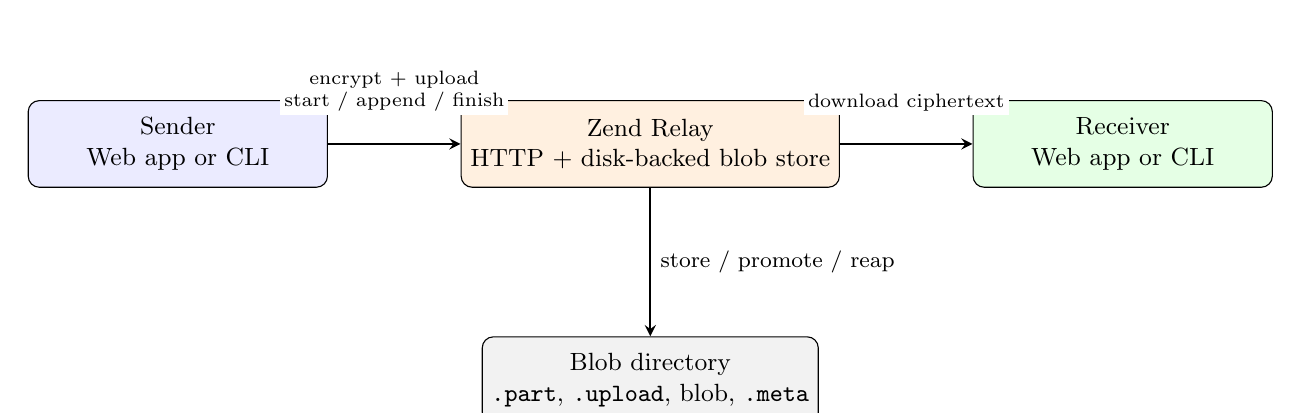
\begin{tikzpicture}[
    box/.style={draw, rounded corners, minimum width=3.8cm, minimum height=1.1cm, align=center, font=\small},
    arr/.style={->, thick, >=stealth}
]
    \node[box, fill=blue!8] (sender) at (-6.0,0) {Sender\\Web app or CLI};
    \node[box, fill=orange!12] (relay) at (0,0) {Zend Relay\\HTTP + disk-backed blob store};
    \node[box, fill=green!10] (receiver) at (6.0,0) {Receiver\\Web app or CLI};
    \node[box, fill=gray!10] (disk) at (0,-3) {Blob directory\\\texttt{.part}, \texttt{.upload}, blob, \texttt{.meta}};

    \draw[arr] (sender) -- node[pos=0.5, above=10pt, align=center, font=\scriptsize, fill=white, inner sep=1.5pt] {encrypt + upload\\start / append / finish} (relay);
    \draw[arr] (relay) -- node[right,font=\footnotesize] {store / promote / reap} (disk);
    \draw[arr] (relay) -- node[pos=0.5, above=10pt, align=center, font=\scriptsize, fill=white, inner sep=1.5pt] {download ciphertext} (receiver);
\end{tikzpicture}
\end{center}

\subsection{Flow Summary}

\begin{enumerate}
    \item The sender chooses a file.
    \item The client generates a random 32-byte key locally.
    \item The file is packetized, optionally compressed per chunk, encrypted, and tagged with a whole-file integrity record.
    \item Ciphertext is uploaded to the relay in ordered append requests.
    \item The sender shares a link of the form \texttt{/d/\{id\}\#\{key\}}.
    \item The recipient downloads the ciphertext blob.
    \item The client decrypts the file and verifies final size and SHA-256 integrity.
    \item The relay deletes the stored blob after a successful download.
\end{enumerate}

\section{Direct CLI Flow}

The CLI also supports a separate direct-transfer mode where one machine connects directly to another over TCP.

\begin{itemize}[leftmargin=1.5cm]
    \item The receiver listens on a TCP port.
    \item The sender connects directly.
    \item The peers perform an X25519-based handshake.
    \item File chunks are encrypted and transferred over the established channel.
\end{itemize}

\notebox{The direct CLI flow is conceptually separate from the relay-backed flow. The relay-backed path uses a locally generated shared-file key embedded in the URL fragment, while the direct path uses an interactive key exchange.}

%==============================================================================
\chapter{Trust Boundaries and Security Model}
%==============================================================================

\section{What the Relay Should Not Learn}

In the relay-backed design, the relay should not learn:

\begin{itemize}[leftmargin=1.5cm]
    \item the plaintext file contents
    \item the file encryption key
    \item the decrypted filename, unless a client leaks it elsewhere
\end{itemize}

This is achieved by encrypting the file before upload and placing the decryption key in the URL fragment, which browsers do not send as part of HTTP requests.

\section{What the Relay Still Learns}

The relay can still observe:

\begin{itemize}[leftmargin=1.5cm]
    \item upload and download timing
    \item blob size
    \item client IP information
    \item request paths and route usage
    \item whether a blob exists, has expired, or has already been consumed
\end{itemize}

\section{Blob Integrity}

The shared protocol code includes an integrity packet containing:

\begin{itemize}[leftmargin=1.5cm]
    \item the final plaintext size
    \item the SHA-256 digest of the final plaintext
\end{itemize}

The decrypt path only treats a file as complete after:

\begin{enumerate}
    \item all frames have been processed in order
    \item authenticated decryption has succeeded for each packet
    \item the final plaintext size matches
    \item the final plaintext hash matches
\end{enumerate}

\section{Operational Safety Properties in the Current Relay}

The current relay implementation enforces several narrow but important safety rules:

\begin{itemize}[leftmargin=1.5cm]
    \item upload appends must arrive strictly in sequence
    \item uploads are capped by total size and per-append size
    \item completion requires the correct upload token
    \item deletion requires the correct blob token
    \item rate limits are applied per IP and per route class
    \item completed blobs and abandoned uploads are reaped on TTL
\end{itemize}

\warningbox{These properties improve safety and abuse resistance, but they do not amount to a formal security audit. Anyone deploying the project for serious use should still review the code and threat model directly.}

%==============================================================================
\chapter{Protocol Notes}
%==============================================================================

\section{Shared Blob Format}

The relay-backed path uses a shared encrypted blob format implemented in Zig and reused by the CLI and WASM targets.

The blob format currently includes:

\begin{itemize}[leftmargin=1.5cm]
    \item encrypted metadata packet with filename and total plaintext size
    \item encrypted chunk packets
    \item optional Huffman compression applied on a chunk-by-chunk basis when it reduces size
    \item encrypted integrity packet with plaintext size and SHA-256 digest
    \item encrypted DONE packet
\end{itemize}

\section{Why the Shared Format Matters}

This shared implementation is one of the strongest consistency points in the current codebase:

\begin{itemize}[leftmargin=1.5cm]
    \item the browser client and relay-aware CLI speak the same format
    \item integrity behavior is not duplicated in separate language implementations
    \item protocol-level tests can cover behavior that matters to multiple clients at once
\end{itemize}

%==============================================================================
\chapter{Current Limits}
%==============================================================================

\section{What the System Already Does Well}

\begin{itemize}[leftmargin=1.5cm]
    \item client-side encryption for relay-backed sharing
    \item relay-side storage of ciphertext rather than plaintext
    \item single-use relay download semantics
    \item cleanup of expired blobs and incomplete uploads
    \item shared protocol logic across CLI and browser paths
    \item CI-backed test and build checks
\end{itemize}

\section{What Is Intentionally Not Claimed}

The current system is not presented as:

\begin{itemize}[leftmargin=1.5cm]
    \item an anonymity system
    \item a synchronized cloud drive
    \item a multi-user storage platform
    \item a formally audited cryptographic product
    \item a system with hidden access patterns or hidden metadata
\end{itemize}

\section{Known Technical Tradeoffs}

\begin{itemize}[leftmargin=1.5cm]
    \item The relay download route currently reads the full blob into memory before responding.
    \item The web app currently has its own UI-level file size cap.
    \item Configuration style still differs somewhat between the relay, the web app, and the CLI.
    \item The direct peer-to-peer CLI mode does not attempt NAT traversal.
\end{itemize}

%==============================================================================
\chapter{Verification and Maintenance}
%==============================================================================

\section{Current Verification Story}

The repository now includes:

\begin{itemize}[leftmargin=1.5cm]
    \item RFC-vector tests for low-level crypto primitives
    \item protocol tests for round-trip behavior, tamper detection, and truncation handling
    \item relay utility tests for ID validation, cleanup helpers, and rate limiting
    \item end-to-end relay tests covering upload, finish, download, consume-on-read, and token-protected deletion
    \item CI jobs for Zig tests/checks and web lint/build
\end{itemize}

\section{Practical Verification Commands}

\begin{lstlisting}[language=bash]
zig build test
zig build check
cd apps/web && pnpm lint && pnpm build
\end{lstlisting}

\tipbox{The project is at its best when the README, CI workflow, and these commands all tell the same story. If one of them changes, the others should be updated in the same pull request.}

\end{document}
